\documentclass[11pt]{article}
\usepackage{graphicx}
\usepackage{amssymb}
\usepackage{epstopdf}
\DeclareGraphicsRule{.tif}{png}{.png}{`convert #1 `dirname #1`/`basename #1 .tif`.png}

\textwidth = 6.5 in
\textheight = 9 in
\oddsidemargin = 0.0 in
\evensidemargin = 0.0 in
\topmargin = 0.0 in
\headheight = 0.0 in
\headsep = 0.0 in

\newcommand{\tarsqi}{T{\sc arsqi}}
\newcommand{\tag}[1]{$<$#1$>$}

\begin{document}


\title{TARSQI Toolkit Specifications}
\author{Marc Verhagen}

\maketitle

This document lays out the speficifcations and the high-level design for the \tarsqi\ Toolkit. It also contains pointers on where the current code needs to be changed. The first section introduces the core idea of the toolkit, lists the most important requirements, and gives a high-level overview. Section 2 describes the document model, one of the main components of the toolkit. Section 3 describes the core TARSQI processing components. The graphical user interface is described in section 4.
 

\section{Introduction}
%---------------------------------------------------------------------------

The \tarsqi\ Toolkit provides one-stop shopping for all temporal processing needs. It takes a variety of texts, pre-processes them, and applies several kinds of temporal processing. The Aquaint Phase II TARSQI project has developed various temporal processing components: (i) {\em GUTime} extracts temporal expressions and assigns normalized values, (ii) {\em Evita} extracts events, (iii) {\em Slinket} extracts subordination  relations, (iv) {\em S2T} assigns temporal relations to subordination relations, (v) {\em Blinker} uses hand-written rules to generate local temporal relations, (vi) {\em the classifier} is a MaxEnt machine learning modal that generates temporal links, and (vii) {\em SputLink} applies temporal closure. The toolkit integrates these components in one environment. 


\subsection{Requirements}

We have adopted the following requirements for the \tarsqi\ Toolkit:

\begin{itemize}

\item Easy to use: it should be easy to install and run on major platforms, functionality is available through a graphical user interface.
\item Integration: all processing components are integrated into a single environment.
\item Standards: the toolkit uses standard programming languages, Python is chosen as the core language.
\item Speed: ability to process one thousand average-sized newswire documents in less than half an hour on an entry-level desktop computer.
\item Robustness: the toolkit should deal with a wide variety of input texts and not break on any kind of textual input.

\end{itemize}

The toolkit should run on the major operating systems (Linux, Windows, Mac OSX) and installation should be simple and not require any additional installations. The only exception is that the toolkit requires version 2.3 of Python, which was first released in 2003. Using an earlier version of Python would be problematic since the GUI requires version 2.3. Python come pre-installed on Linux and Mac OSX, an easy installer for Windows is available at ActiveState.com.

The requirements have a couple of repercussions for the current code base. First, standardization on Python runs afoul with some components that are now implemented in Perl (glue scripts, tokenizer, chunker, GUTime and Sputlink). These will be re-implemented in Python, making integration easier. Second, all components are now offered as standalone scripts and can only take input from files and write output to files. With the toolkit, all programs are integrated and file input and output should be optional. Third, it now takes about 90 minutes to process a thousand documents, but the amount of data that the toolkit must be able to process has to be several orders of magnitude higher. A substantial speedup is required to allow processing of tens or hundreds of thousands documents.


\subsection{Toolkit Design Overview}

At the highest level of abstraction, the toolkit can be viewed as having two main components: the document model and the core processor.

\begin{quote}
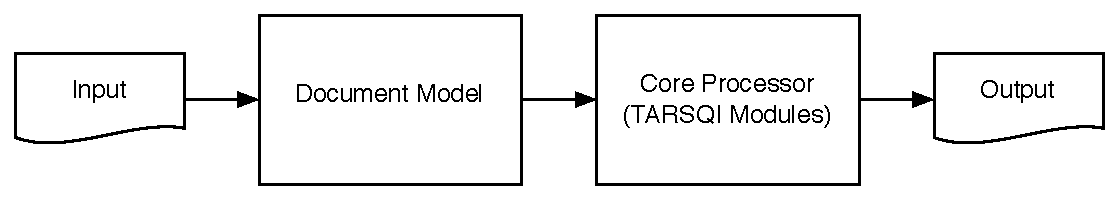
\includegraphics[width=4in]{images/architecture1.pdf} 
\end{quote}

The {\em Document Model} is responsible for dealing with the peculiarities of the data source. It reads in the document with an XML parser (first converting the document into trivial XML if needed), sets parameters for the core processor, and feeds the appropriate fragment of the document into the core processor. The input to the document model is the document with an associated document type. The document type indicates the format of the document as well as its genre. The {\em Core Processor} controls access to the \tarsqi\ modules. It takes parameters and data from the document model and feeds the data through the appropriate temporal processing components including pre-processing components (tokenizing, tagging and chunking), time and event recognition (GUTime and Evita), modal parsing (Slinket and S2T) and temporal parsing (GUTenlink/Blinker, TLink Classifer and Sputlink).


\section{The Document Model}
%---------------------------------------------------------------------------

The document model handles all source and genre specific peculiarities of a document: setting processing parameters, parsing meta data, reading the document and selecting the part of the document that needs to be temporally processed.

\begin{quote}
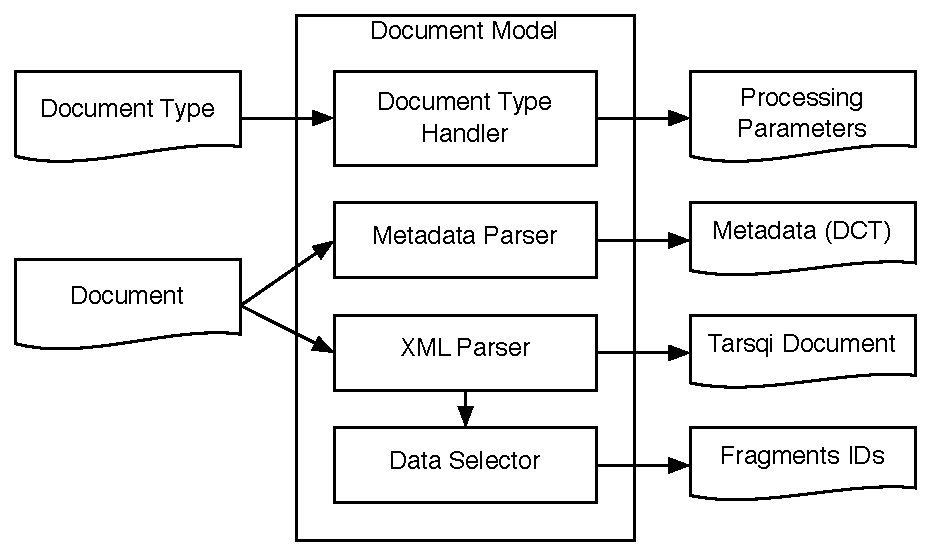
\includegraphics[width=4in]{images/architecture2.pdf} 
\end{quote}

The {\em Document Type Handler} takes the input type and creates a set of parameters. The input type is an identifier like {\tt preprocessed-timebank}, {\tt atee-doc} or {\tt plain-text}. The main parameters to be set are the processing chain and the genre, but the latter is not used until we actually have a genre that is not newswire text. The processing chain is encoded as a list that stipulates what components need to be applied. For example, for the identifier {\tt preprocessed-timebank}, the processing chain parameter may be set as follows:

\begin{quote}
{\tt [ gutime ; evita ; slinket ; s2t ; blinker ; classifier ]}
\end{quote}

The ideal situation is that all components work on a shared in-memory structure, but it is very likely that some components, like the tagger and the classifier, will not be implemented in Python and may need to work with file input and output. For these cases, the processing chain should specify what the input and output files are. Note that when the GUI is available, the processing chain parameter will actually be constructed by the user by checking off what components need to be applied. The document type handler also determines what dictionaries should be used by the \tarsqi\ components, this however will not come to pass till year two of the toolkit project.

The {\em Metadata Parser} scans the document for meta data like document creation time (DCT), source, author, meta tags, etcetera. For temporal processing purposes, the DCT is the most important meta data element. This component is likely to be the component that is most dependent on the actual format of the input document and would need to be implemented for many data formats. 

The {\em XML Parser} is as light-weight as possible and should deal with any XML data and make no assumptions as to what tags to expect. Note that the input is not necessarily XML input. For those cases, the document model includes a step that creates a trivial XML file where all text is wrapped into at least a \tag{DOC} tag, but other tags can be used to make document structure explicit. The {\em XML Parser} creates a Document object with at least the following data structures:

\begin{itemize}

\item
A linked list of document elements. Each document element can be an opening tag, a closing tag, a set of character data, a processing instruction, the xml declaration, or any other element. A document element knows what the previous and next elements are. It also knows how to find its content and its closing tag, delete itself, insert an element before or after itself, and wrap itself inside of a new tag.

\item
A dictionary indexed on tag names where the values are lists of document elements of the opening tags. This dictionary allows quick access to any tag and its content. For example, we can access the first \tag{EVENT} tag by referring to {\tt document.tag\_dictionary['EVENT'][0]} and with this tag we can then access the location of the first event tag in the linked list of the document.

\end{itemize}

Other dictionaries may be added as needed to speed up access. It may for example be useful to have quick access to closing tags in case we insert new tags before this closing tag and we want to avoid the potentially costly route via the opening tag. There should only be one XML parser in the toolkit. If data need to be XML-parsed twice because some component only works with file input and output, then the same parser is used. Also, the parser introduces no structure that could be obtained from chunking tags in the document, this is the responsibility of the core processor.

The last component of the document model, the {\em Data Selector}, has a limited function. It simply identifies the tag or tags that contain the part of the document that needs to be processed temporally. Conceptually, the data selector can be considered to be part of the document type handler.

The main Python class that implements the document model is {\em DocumentModel}. It contains classes {\em DocTypeHandler}, {\em MetadataParser}, and {\em DataSelector}. An instance of {\em DocumentModel} does not necessarily contain an {\em XmlParser} since the XML parser is a general parser that works for any document type and because it is safest to initialize a new parser each time one is needed. Here is a code fragment that illustrates how components of the document model are incorporated in or used by the main {\em DocumentModel} class:

\begin{quote}
\begin{verbatim}
class DocumentModel:
    def __init__(self):
        self.doc_type_handler = DocTypeHandler()
        self.metadata_parser = MetadataParser()
        self.data_selector = DataSelector()
    def read_document(self, filename):
        parser = XmlParser()
        self.document = parser.parse(filename)
\end{verbatim}
\end{quote}

For each data source a new subclass of DocumentModel can be defined, one that may refer to subclasses of the embedded classes:

\begin{quote}
\begin{verbatim}
class TimeBankModel(DocumentModel):
    def __init__(self):
        self.doc_type_handler = TimebankDocTypeHandler()
        self.metadata_parser = TimebankMetadataParser()
        self.data_selector = TimebankDataSelector()
\end{verbatim}
\end{quote}

All code is defined on the DocumentModel class, differences on how TimeBank data need to be processed are all implemented on the embedded classes. There is an alternative approach where there are no subclasses of DocumentModel, but where initialization of a DocumentModel instance takes parameters:

\begin{quote}
\begin{verbatim}
class DocumentModel:
    def __init__(self,doc_type_handler, metadata_parser, data_selector):
        self.doc_type_handler = doc_type_handler()
        self.metadata_parser = metadata_parser()
        self.data_selector = data_selector()
        
timebank_model = DocumentModel(
                     TimebankDocumentTypeHandler, 
                     TimebankMetadataParser, 
                     TimebankDataSelector)
\end{verbatim}
\end{quote}

The first approach is more flexible because it allows subclasses of DocumentModel to override methods (note that this is not the intention, but it may be necessary or convenient anyway). Some likely subclasses of {\em DocumentModel} are {\em TimebankModel}, {\em PreprocessedTimebankModel}, {\em AteeModel}, {\em PlainTextModel} etcetera.

What class is used to deal with a document depends on the document type identifier. So the document model will always be embedded in a wrapper that determines what document model to use. The document model does not contain a Tarsqi core processor, but it hands whatever is needed by the core processor to the core processor. Here's some Python code that takes care of the top-level processing (note that TarsqiControl is the main class of the core processor, as explained in the next section):

\begin{quote}
\begin{verbatim}
# determine what document model to use, given the document type
doc_model = select_model(document_type)
# take the input file and set instance variables for processing parameters, 
# meta_data, parsed document, and fragment IDs
doc_model.process(inputfile)  
# initialize the core processor, using data from the document model
# and process the file according to those settings
core_processor = TarsqiControl(doc_model)
core_processor.process()
\end{verbatim}
\end{quote}




\section{The Core Processor}
%---------------------------------------------------------------------------

The document model hides all particulars of a data source from the core processor. The core processor can therefore concentrate on the temporal processing of a document. It receives four inputs from the document model: processing parameters, metadata, an XML tree (implemented as a Document object) and a set of fragment IDs that refer to parts of the XML tree.

\begin{quote}
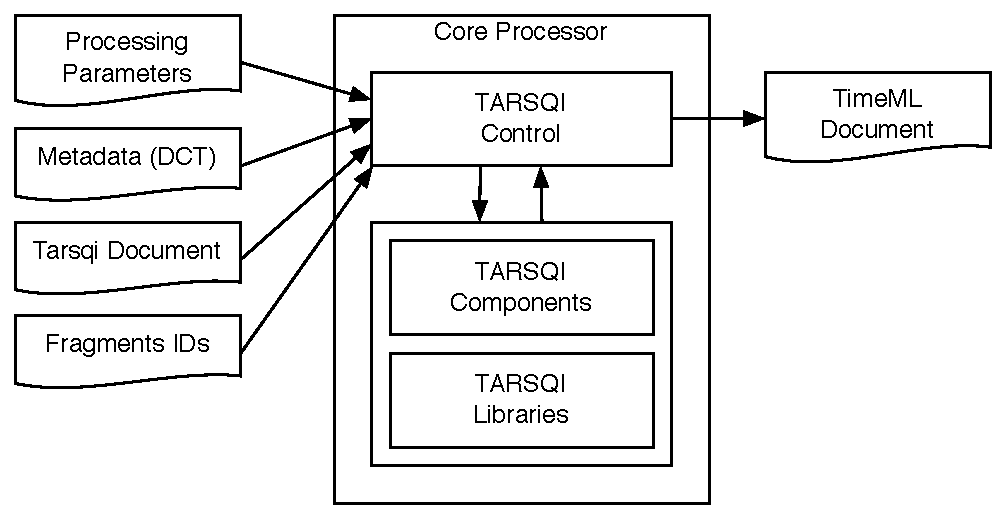
\includegraphics[width=4in]{images/architecture3.pdf} 
\end{quote}

The core processor has three components: {\em TARSQI Control}, {\em TARSQI Components} and {\em TARSQI Libraries}. The controller reads the processing parameters. One of the parameters, the processing chain, determines what \tarsqi\ components will be selected by the controller and applied to the elements of the document identified by the fragment IDs. The controller will provide metadata as needed (GUTime for example will require the DCT). The processing parameters also determine what libraries will be used by the \tarsqi\ components.

All components ideally work on the same in-memory data structure. If a component can not be integrated this way (which may be the case for the tagger and the TLINK classifier), then a wrapper needs to be defined that uses the in-memory data structures to feed the wrapped component, this wrapper would also use the filenames provided by the processing chain parameter. Alternatively, the wrapper could simply know where the file sand box for the embedded component is and read and write from there. In that case, there is no need for the document model to define where the input and output files for the wrapped components are. 


\subsection{TARSQI Control}

The core processor contains the \tarsqi\ components, the \tarsqi{} libraries and a control class that ties everything together. The {\em TarsqiControl} class is responsible for:

\begin{itemize}
\item Importing data from the document model.
\item Selecting and loading the appropriate dictionaries and patterns sets.
\item Maintaining a shared document resource, originally created by the XML praser of the document model.
\item Handing data from the shared document resource to individual Tarsqi components.
\item Transforming those data if needed (for example, Evita and Slinket do not accept a flat list of document elements, but require a shallow tree that contains chunking information).
\item Ensuring that tags added by components find their way into the shared resource, this is not needed for those components that manipulate the shared resource directly.
\end{itemize}

The data come in from the document model as a linked list of document elements and the parts of the linked list that need to be processed are given as a list of document elements or document element IDs. These lists of document elements are fed into the components. In some cases, as with the tokenizer for example, the list may contain only one element with character data, in other cases, like with Evita, the list will be structured further before it is given to the component for processing. We will now describe all the \tarsqi\ components as they are, each followed by specifications on how they need to be changed. 

\subsection{Pre-processing}

Currently, the toolkit includes a Perl tokenizer, the IMS TreeTagger (implemented in Java with a Python wrapper), a Perl chunker, and various Python and Perl glue scripts. This works, but needs to be improved. Somewhere in our proposal, we indicated that it should be easy to slot in different preprocessing components. The tokenizer and chunker will both be reimplemented in Python. The input to the pre-processing stage is an in-memory Python data structure, namely a slice from the TarsqiDocument created by the XML parser.

\subsubsection{Tokenizer}

The requirements for the tokenizer are as follows:

\begin{itemize}

\item Creates output with $<$lex$>$ tags and provides an option to add $<$s$>$ tags

\item Does not change the text, except by adding tags, removing these tags should result in the original input

\item Can output tokenized text in alternative formats, depending on what the tagger requires; this flexibility will take away the need for the Python glue scripts

\item Protects certain strings, like opening XML tags and URLs, as single tokens.

\item Allows input that already has sentence tags

\item Input and output are either a Python data structure or a file.

\end{itemize}

The current tokenizer does not meet all these requirements, in fact, it only meets a few. Part of the requirements should be a clear definition of what a token is. 
 
 
\subsubsection{Tagger}

The current tagger of record is the IMS TreeTagger. It comes with a Python wrapper that makes it possible to repeatedly call the tagger from Python without reloading the tagger dictionaries each time a file is tagged. Currently, it does still rely on file input and output, but this may possibly be changed by editing the Python wrapper. The main problem with it is that, although it is free for use in academic settings, we do not have permission to distribute the TreeTagger with the toolkit. A long email exchange with IMS has not resolved this issue. We could either try to again resolve this with IMS, or investigate the use of a more freely available Python tagger. 


\subsubsection{Chunker}

The chunker should add \tag{NG}, \tag{VG}, and \tag{AG} tags to identify noun groups, verb groups and adjective groups. The current Perl chunker should be reimplemented in Python and be able to take text with $<$lex$>$ and $<$s$>$ tags. It should also introduce adjective chunks.


\subsection{GUTime}

GUTime is the component that adds information on temporal expressions by adding TIMEX3 tags. It consists of several components. The core components, {\tt TimeTag.pl} and {\tt TempEx.pm}, are the original TempEx scripts from MITRE (George Wilson and Inderjeet Mani). All other scripts are written by Georgetown University. 

{\tt GUTime-Evita.pl} is a wrapper around TimeTag.pl that tries to find the document creation time and creates the input file for TimeTag.pl by stripping all tags except for $<$lex$>$ and $<$s$>$ tags. After running TimeTag.pl, it calls some other scripts for further processing and to glue everything together again: (i) {\tt postTempEx.pl} adds some temporal functions but these never seem to make it to the output, (ii) {\tt merge-gutime.pl} takes the original input document and the Tempex output and merges the tags together, and (iii) {\tt TagOrder.pl} fixes some of the crossing tags introduced by the previous script.

% Problems with GUTime

GUTime is one of our weaker components in the sense that it is the least robust. It easily breaks on any kind of xml input, it seems to deal decently with $<$lex$>$ and $<$s$>$ tags as well as the tags added by Evita, but beyond that every added tag can cause trouble. The merging scripts are the most problematic. {\tt merge-gutime.pl} liberally introduces crossing tags and only few of these are resolved by {\tt TagOrder.pl}. It was very hard to integrate GUTime due to the unreliability of the merging phase. The system had to pick 'clean' components from input files and feed them separately into GUTime, thereby increasing the number of system calls and file I/O as much as 10 to 100 times (this was admitttedly not a very sophisticated way to do it). In addition, {\tt GUTime-Evita.pl}, itself a system call from the toolkit, uses three more system calls to do its bidding.

TempEx was state-of-the-art almost a decade ago, but cannot be maintained because essentially it is one huge conditional statement with massive regular expressions thrown in. It is also probably slower than it should be.

% Changes

Eventually, we will ditch all of GUTime, but we have to deal with the merging problems soon. The mid-term goal is to have one Python script wrapped around the core components, and have this script take over all functionality from the Georgetown Perl scripts. Things that need to be done are (in order of urgency):

\begin{enumerate}

\item Replace {\tt merge-gutime.pl} and {\tt TagOrder.pl} with a Python script

\item The name {\tt GUTime-Evita.pl} is silly, it was named that way because it was a version of GUTime that could run on output of Evita, but should be renamed now it applies before Evita 

\item A large part of {\tt GUTime-Evita.pl} is about finding the document creation time, this code should be moved to the document model

\item Find a new name for GUTime (current working name: Brandeis University Time Tagger; other proposals: Brute, BRUT...)

\item Fully replace {\tt GUTime-Evita.pl} with python code

\item Replace {\tt TimeTag.pl} and {\tt Tempex.pm} with Python code and let it use the unified pattern language that will be defined for all rule-based modules

\end{enumerate}

The Python script that takes over the tag merging of two documents can use the following strategy: (1) parse both documents (doc1 with the \tag{TIMEX3} tags and doc2 with all tags from the input)  using the XML parser, (2) line up the \tag{lex} tags with each other and give them identical IDs across the two documents, (3) for each \tag{TIMEX3} tag in doc1, get the list of included \tag{lex} tags, (4) get the sequence of of tags from doc2 where the opening tag of the first \tag{lex} is the first item and the closing tag of the last \tag{lex} tag the last, (5) wrap this sequence in a temporary tag and check whether it is well-formed XML, and (6) if it is, wrap the sequence in doc 2 in the \tag{TIMEX3} tag. Note that step (1) is not necessary if the data structures are already in memory. If step (5) fails, some strategies can be employed to try to take a larger sequence from doc2: including opening tags to the left that match a stranded closing tag inside the original sequence, or taking in a closing tag on the right that matches a stranded opening tag in the original sequence.


\subsection{Evita}

Evita generates event tags by looping through all elements of a sentence and checking whether these elements could be an event. The elements are expected to be chunks in the case where we are looking for a verbal or nominal event or tokens in case we're looking for an adjectival event. When a chunk is a confirmed event chunk, then an event tag is wrapped around the head of the chunk, where head is defined as the rightmost element. \tag{EVENT} tags are wrapped inside of \tag{lex} tags. Evita currently takes its input from a file and uses its own XML parser to create the data structure it needs.

It is clear that chunking information is essential for event recognition and the flat list of document elements provided by the document model is not ideal for Evita. Recall that the \tarsqi\ control module is responsible for providing transformed document resources as required by the \tarsqi\ components. Take for example the document resource for the short sentence "Fido barks". It is initially created by the XML parser as a linked list of document elements:

\begin{quote}
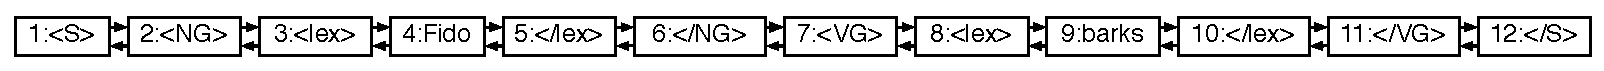
\includegraphics[width=6.0in]{images/doc_resource1.pdf} 
\end{quote}

The resource transformer turns this flat list into a tree structure, where the shape of the tree is determined by the chunking tags: 

\begin{quote}
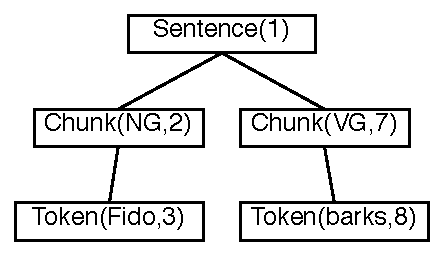
\includegraphics[width=2.0in]{images/doc_resource2.pdf} 
\end{quote}

The thing to note about this tree is that it contains pointers back to the original linked list of document elements. Therefore, when Evita decides that the verb chunk contains an event, then the document element contained in the head token of the chunk, in this case the one with the identifier~8, can be accessed and an \tag{EVENT} tag can be wrapped around that document element and a makeinstance lement can be added immediately after (note that this assumes that the event tag is wrapped around the lex tag, which is different from the current situation).

\begin{quote}
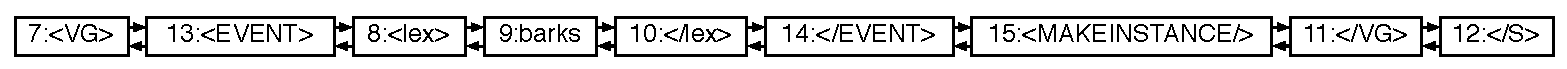
\includegraphics[width=6.0in]{images/doc_resource3.pdf} 
\end{quote}

The tree representation does not need to be changed, but constituents in it will receive extra tags. For example, the node for the token {\em barks} will now get a feature saying that the token is also an event, with a pointer to the event tag in the linked list.

\medskip\noindent
Evita is now a standalone scripts that uses its own XML parser to create the input. Instead, Evita should rely for its input on the XML parser from the document model and the resource transformer from the \tarsqi\ control module. Similarly, Evita should not use its own idiosyncratic way to write output but only manipulate the shared data resource, leaving the creation of file output to other modules.

Another needed change to Evita is that it should use the unified pattern language mentioned before in the section on GUTime. This however is not required till the second year of the project


\subsection{Slinket}

NOT YET WRITTEN

%Another needed change to Slinket is that it should use the unified pattern language. Again, this is not a requirement in the first year of the project.


\subsection{S2T}

NOT YET WRITTEN

%Another needed change to S2T is that it should use the unified pattern language mentioned before in the section on GUTime. This however is not a requirement till the second year of the project, but S2T will have to eliminate the hard-wired patterns from the code.

\subsection{GUTenLink/BLinker}

NOT YET WRITTEN

\subsection{The Classifier}

NOT YET WRITTEN

\subsection{SputLink}

SputLink is the temporal closure component based on the interval algebra of James Allen. Temporal relations between intervals (events and times) are maintained in a graph where the nodes are the intervals and the arcs are labeled by arbitrary disjunctions over the thirteen basic relations. When a new temporal relation between two intervals is added, all consequences are generated by computing the transitive closure of the temporal relations. Each new fact adds a constraint about how its two intervals could be related, which may in turn introduce new constraints between other intervals through the transitivity rules governing the temporal relations. Allen's algebra runs in polynomial time but it is nowhere near linear: it is O(n$^3$) to the number of intervals. The main problem is that it is not guaranteed to find all inconsistencies. To solve that, SputLink adopts restrictions on the set of allowed disjunctions from the point algebra of Villain, Kautz and van Beek.

Temporal closure is by far the slowest of all toolkti components, as is illustrated in the table below, which gives the running times in second for all components on the entire TimeBank corpus.

\begin{quote}
\begin{tabular}{|l|r|}
\hline
Tokenizer 					&   4 \\
IMS TreeTagger 				&  11 \\
Chunker				 		&   7 \\
GUTime 						&  98 \\
Evita 						&  41 \\
Slinket						&  45 \\
S2T							&  24 \\
Classifier 					&  88 \\
Merging, using sputlink		& 496 \\
\hline
TOTAL 						& 814 \\
\hline
\end{tabular}
\end{quote}

The goal is to make the toolkit at least two to four times faster, this cannot be done without substantially improving the speed of SputLink. Being cubed in processing time, SputLink really struggles with long documents. Let's say that, hypothetically, a document with 10 events takes one second to process. We then see the following extrapolated processing times for documents of different sizes (with sized measured in number of events):

\begin{quote}
\begin{tabular}{|r|r|}
\hline
size	& time\\
\hline
 10  	&    1 \\
 20		&    8 \\
 50		&  125 \\
100		& 1000 \\
\hline
\end{tabular}
\end{quote}

It is actually already impractical to run closure on some of the largest TimeBank documents. SputLink's processing speed can to be improved in two ways:

\begin{enumerate}
\item optimization of code
\item changes to the algorithm
\end{enumerate}

SputLink is now implemented in Perl, but there is a Java version as well as a bare-bones Python version. Using the Python version makes it easier to integrate closure with other toolkit components and gives us a couple of options for potentially significant optimization: using data structures that are implemented as C extensions in the standard library, and implementing the most processing intensive parts in C.

This optimization will obviously not change the nature of the algorithm and larger documents will still be impractical. We need to put a different bound on the time complexity. This can be done by using {\em partitioned closure}. With partitioned closure, closure will not run on the entire graph but on set of subgraphs. And if the size of the subgraphs is bounded to some fixed value, then the time complexity of closure will be O(n) rather then O(n$^3$). Suppose we have a graph with nine events:

\begin{quote}
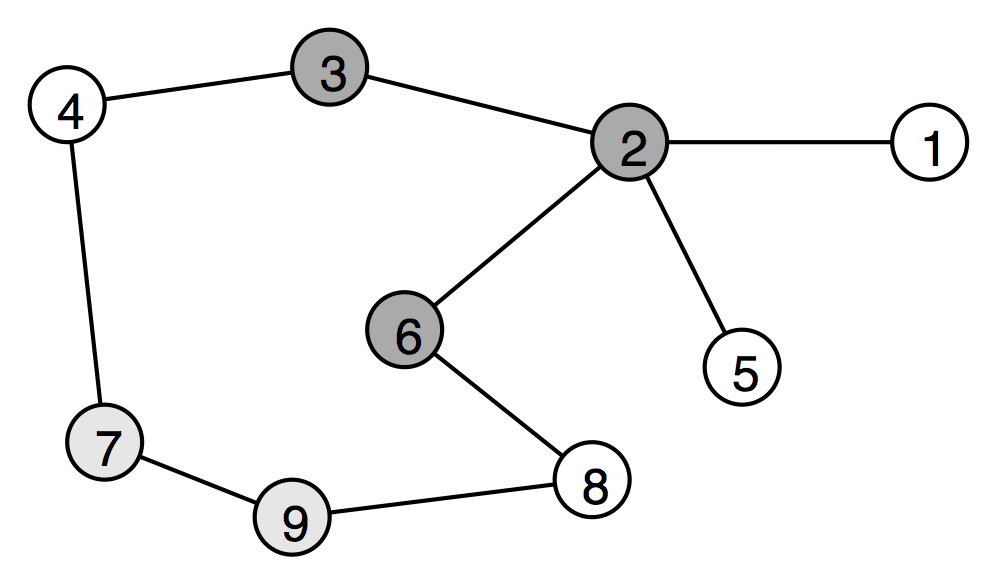
\includegraphics[width=2.5in]{images/closure1.png} 
\end{quote}

And suppose we have set a size limit of 3 to the size of a graph partition. We now need to cut the graph in three.

\begin{quote}
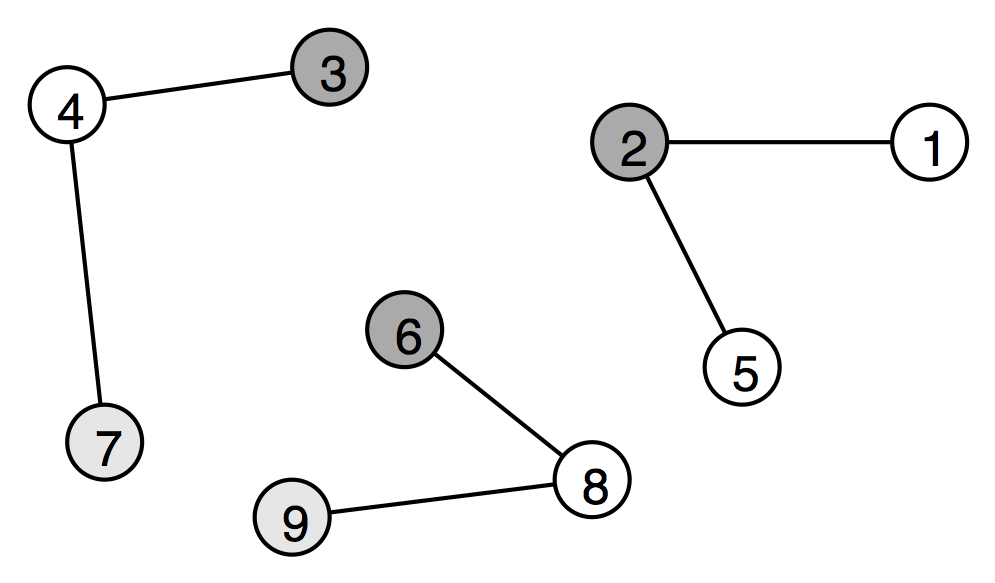
\includegraphics[width=2.5in]{images/closure2.png} 
\end{quote}

But now we have three unconnected graphs and we will never be able to build a temporal picture of the whole document, which is not acceptable. We need to introduce a further subgraph that contains the temporal relations between the nodes where the cuts were made.

\begin{quote}
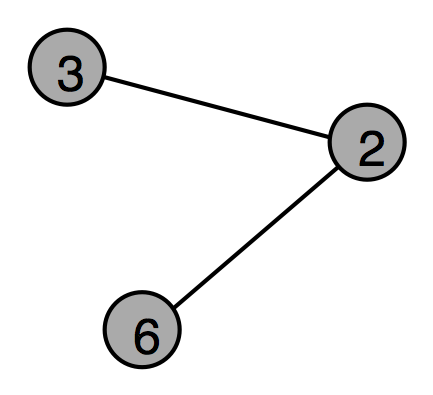
\includegraphics[width=1.2in]{images/closure3.png} 
\end{quote}

Now we can run closure on all four subgraphs without worrying about the size of the entire disk. 

\newpage
A couple of things should be noted:

\begin{itemize}
\item we have lost some information because we needed to cut the link between 6 and 7
\item we need to make sure that we still catch inconsistencies
\item we need a procedure to find good partitions
\end{itemize}

MORE TO FOLLOW


\subsection{TLINK Merging}

NOT YET WRITTEN

\subsection{TARSQI Libraries}

NOT YET WRITTEN


\section{The Graphical User Interface}
%---------------------------------------------------------------------------

NOT YET WRITTEN




 \end{document} 